\chapter{Experimentación: modelos \\ y entrenamiento}

En este capítulo usaremos todos los conceptos vistos en los capítulos anteriores para justificar las elecciones de los diferentes modelos, hablaremos de las características principales de los mismos y finalmente entraremos en la fase del entrenamiento y los resultados de dichos modelos.

\begin{figure}[h]
	\centering
	\includegraphics[width=.9\textwidth]{media/gpt-fine-tune.pdf}
	\caption{Diagrama resumen del ajuste de los pesos del GPT2}
	\label{fig:fine-tune-gpt}
\end{figure}

En la figura \ref{fig:fine-tune-gpt} podemos ver un breve resumen de las diferentes tareas de las que se compone el entrenamiento del modelo. Pasaremos a explicar en profundidad cada una de esas subtareas en las siguientes secciones.


\section{Experimentación}
En esta sección describiremos los diferentes pasos que fue necesario acometer para el entrenamiento del modelo del GPT2, el transformer que hemos utilizado para nuestro proyecto.

\subsection{Entrada de los datos}
En primer lugar, debemos ofrecer los datos de entrada al modelo. Estos datos están previamente formateados y unificados, como vimos en la fase de preprocesamiento.

Es importante la adición de las etiquetas \jesitt{<|BOS|>} y \jesitt{<|EOS|>}. Estas etiquetas son las siglas de \textit{begin of sentence} y \textit{end of sentence}. Son marcadores que indican, como es obvio, el inicio y fin de una oración. Estas etiquetas son necesarias para que el modelo entienda cuál es el criterio a partir del cual empieza y acaba una oración.

\subsection{Codificación de los tokens}
Antes de pasar los datos al modelo, debemos codificarlos. Codificar significa obtener un código único en función del token que estemos considerando. La codificación es esencial para estos modelos, ya que ofrece una representación matemática de las palabras. La codificación de los tokens se efectúa mediante un diccionario preentrenado, de forma que la codificación decodificación sean consistentes, dado un modelo determinado.


\subsection{Ajuste de los pesos}
Nuestro modelo ya está construido. Esto es, los diseñadores ya han decidido las distintas capas y el orden de estas según hemos visto en las secciones anteriores. Este modelo se nos ofrece preentrenado de forma bastante simple. Tal y como viene en el paquete, es capaz de generar frases con relativo sentido, es decir, de algún modo \textit{sabe hablar}. El ajuste se efectúa como un proceso de aprendizaje no supervisado, en la que exponemos a la red a un conjunto de comentarios de forma que ésta podrá generar nuevos comentarios de la nada que caigan bajo la función de distribución de los comentarios de entrada. 

En nuestro caso, esta \textit{función de distribución} la define nuestro conjunto de datos de informes médicos. Este proceso efectivamente ajusta los pesos de la red de forma que se familiarice al modelo con el vocabulario y expresiones comunes encontradas en nuestro conjunto de datos.

Como sabemos, este proceso es, computacionalmente, extraordinariamente costoso. Debemos calcular el peso de millones de parámetros (117 millones en nuestro caso particular), debido a la magnitud del modelo. Para ello, hemos de tener disponible un equipo con, como mínimo, una tarjeta gráfica decente que nos permita hacer cálculos matriciales en paralelo, operaciones muy comunes en el entrenamiento de las redes neuronales.

Dichos equipos pueden ser muy caros. Para ello, hicimos uso del servicio de clústeres de la UGR, enviando nuestros datos mediante \jesitt{ssh}, entrenando el modelo, y descargándonoslos de vuelta.

\subsection{Guardado del estado del modelo}
Finalmente, una vez entrenado el modelo, lo más importante es guardar su estado. Esto es muy fácil gracias a los métodos provistos por las librerías de deep learning. Este estado se guarda en un archivo, que, generalmente, consta de un diccionario en el que las claves corresponden a los nodos de las capas en sí, es decir, a sus parámetros entrenables, y cuyo valor es el peso de dicho nodo. 

De esta forma, es fácil cargar un modelo \textit{vacío}, un modelo inicializado con pesos nulos o no relevantes, y sustituir dichos valores por los incluidos en el archivo. Esto nos permite volver al estado en el que dejamos al modelo tras el costoso entrenamiento.

\section{Generación de comentarios}

\begin{figure}[h]
	\centering
	\includegraphics[width=.9\textwidth]{media/comment-gen.pdf}
	\caption{Diagrama resumen de la generación de comentarios}
	\label{fig:comment-gen}
\end{figure}

En esta sección hablaremos de la generación de comentarios, una vez nuestro modelo está entrenado y listo para funcionar. 

\subsection{Carga del modelo}
Como indicamos anteriomente, la carga del modelo es realmente sencilla gracias a las librerías que lo hacen posible. Con nuestro archivo con los pesos localizado, podemos cargar de vuelta los pesos relevantes en los parámetros correspondientes de la red, recuperando el estado original. Este estado es el que nos permitirá generar comentarios de forma automática.

\subsection{Sampling y otros métodos de generación de texto}
Ahora que nuestro modelo está listo, podremos generar comentarios de la nada, casi como por \textit{arte de magia}. Aún así, este proceso no es trivial y merece ser aclarado.

Debemos gran parte de esta sección a la magnífica explicación de Patrick von Platen en su publicación \href{https://huggingface.co/blog/how-to-generate}{How to generate text}. Precisamente es uno de los integrantes de Hugging Face, una empresa de código abierto que se dedica a la creación de los diferentes modelos de los que hemos hablado anteriormente, y que nos ha provisto con una manera fácil y accesible de poder utilizar estas herramientas tan potentes.

Existen varias maneras de generar lo que en la jerga se denomina \textit{texto abierto}, es decir, texto libre sin restricciones. Muchos modelos son capaces de hacerlo, aunque nosotros nos centraremos en los métodos que conciernen al GPT2, que es un modelo autorregresivo.

Los modelos autorregresivos asumen que la siguiente palabra a generar se calcula como una función de probabilidad de todas las palabras anteriores, dada una palabra de contexto inicial.

\subsubsection{Greedy and beam search}
La búsqueda voraz obtiene la palabra con mayor probabilidad de todas las opciones dada una palabra inicial. 


\begin{figure}[h]
	\centering

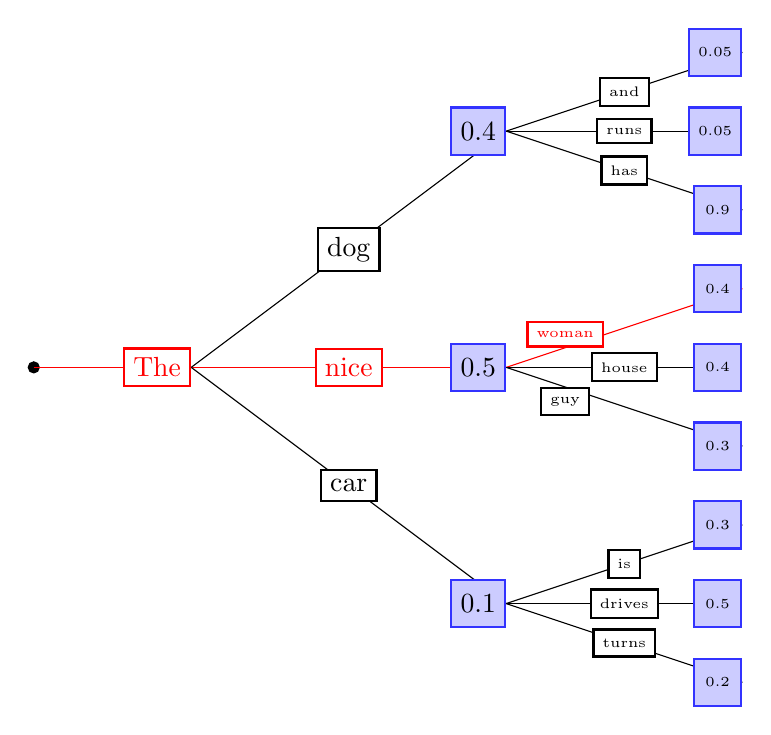
\begin{tikzpicture}
	\tikzstyle{tag}=[shape=rectangle,thick,draw,fill=white,minimum size=0.3cm]
	\tikzstyle{ntag}=[shape=rectangle,thick,draw=blue!80,fill=blue!20,minimum size=0.6cm]

	\filldraw [black] (-4,0) circle (2pt);
	
	
	%%%
	\draw (-2,0) -- node[tag] {dog} (2,3);
	\draw[red] (-2,0) -- node[tag] {nice} (2,0);
	\draw (-2,0) -- node[tag] {car} (2,-3);
	
	\node at (2, 3) [ntag, anchor= east] {0.4};
	\node at (2, 0) [ntag, anchor= east]{0.5};
	\node at (2, -3) [ntag, anchor= east]{0.1};
	
	
	%%%
	\draw[red] (2,0) -- node[tag, near start, anchor=south] {\tiny woman} (5,1);
	\draw (2,0) -- node[tag] {\tiny house} (5,0);
	\draw (2,0) -- node[tag, near start, anchor=north] {\tiny guy} (5,-1);
	
	
	
	\node at (5, 1) [ntag, anchor= east] {\tiny 0.4};
	\node at (5, 0) [ntag, anchor= east]{\tiny 0.4};
	\node at (5, -1) [ntag, anchor= east]{\tiny 0.3};
	
	%%%
	\draw (2,3) -- node[tag] {\tiny and} (5,4);
	\draw (2,3) -- node[tag] {\tiny runs} (5,3);
	\draw (2,3) -- node[tag] {\tiny has} (5,2);
	
	\node at (5, 4) [ntag, anchor= east] {\tiny 0.05};
	\node at (5, 3) [ntag, anchor= east]{\tiny 0.05};
	\node at (5, 2) [ntag, anchor= east]{\tiny 0.9};
	
	%%%
	\draw (2,-3) -- node[tag] {\tiny is} (5,-2);
	\draw (2,-3) -- node[tag] {\tiny drives} (5,-3);
	\draw (2,-3) -- node[tag] {\tiny turns} (5,-4);
	
	\node at (5, -2) [ntag, anchor= east] {\tiny 0.3};
	\node at (5, -3) [ntag, anchor= east]{\tiny 0.5};
	\node at (5, -4) [ntag, anchor= east]{\tiny 0.2};


	\draw[red] (-4,0) -- (-2,0)
	node[tag, anchor=east] {The};
\end{tikzpicture}

	\caption{Ilustración de los pasos que daría el algoritmo greedy, tomando siempre la posibilidad más alta}
	\label{tkz:greedy}
\end{figure}

Dada una palabra inicial que tomamos del usuario, por ejemplo, siempre tomaremos aquella palabra de todas las posibles opciones que más probabilidad tenga de aparecer, dada la palabra anterior. Dichas probabilidades se calculan en el entrenamiento del modelo.

El algoritmo toma siempre la palabra más probable y esto funcionará bien, aunque este algoritmo peca de empezar a repetirse bastante pronto. Esto es, generará secuencias que contienen palabras finales e iniciales similares, por lo que el ciclo empieza de nuevo al escogerse siempre la palabra más probable.



\begin{figure}[h]
	\centering
	
	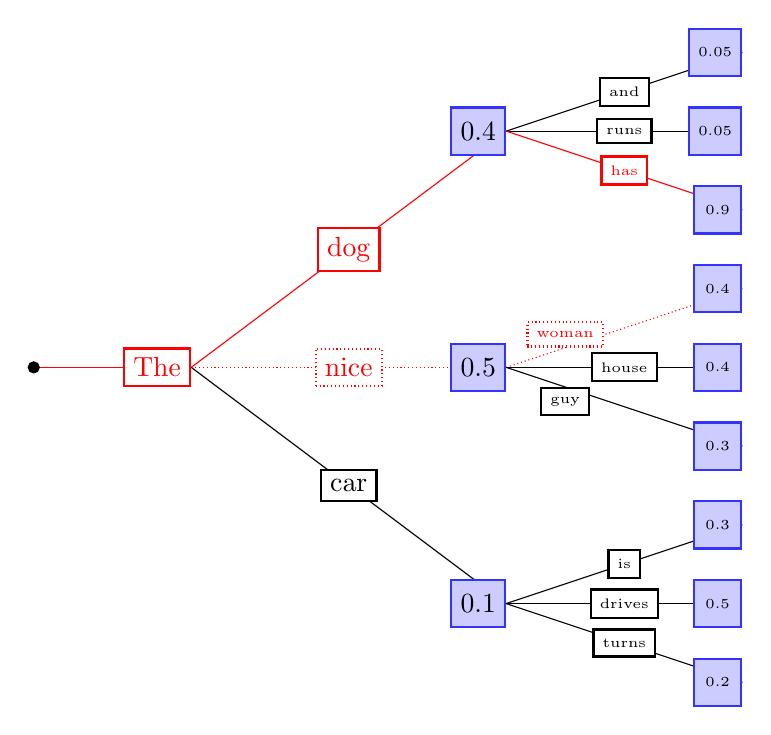
\begin{tikzpicture}
		\tikzstyle{tag}=[shape=rectangle,thick,draw,fill=white,minimum size=0.3cm]
		\tikzstyle{ntag}=[shape=rectangle,thick,draw=blue!80,fill=blue!20,minimum size=0.6cm]
		
		
		\draw[red] (-4,0) -- (-2,0)
		node[tag, anchor=east] {The};
		
		\filldraw [black] (-4,0) circle (2pt);
		
		
		%%%
		\draw[red] (-2,0) -- node[tag] {dog} (2,3);
		\draw[red, densely dotted] (-2,0) -- node[tag] {nice} (2,0);
		\draw (-2,0) -- node[tag] {car} (2,-3);
		
		\node at (2, 3) [ntag, anchor= east] {0.4};
		\node at (2, 0) [ntag, anchor= east]{0.5};
		\node at (2, -3) [ntag, anchor= east]{0.1};
		
		
		%%%
		\draw[red, densely dotted] (2,0) -- node[tag, near start, anchor=south] {\tiny woman} (5,1);
		\draw (2,0) -- node[tag] {\tiny house} (5,0);
		\draw (2,0) -- node[tag, near start, anchor=north] {\tiny guy} (5,-1);
		
		
		
		\node at (5, 1) [ntag, anchor= east] {\tiny 0.4};
		\node at (5, 0) [ntag, anchor= east]{\tiny 0.4};
		\node at (5, -1) [ntag, anchor= east]{\tiny 0.3};
		
		%%%
		\draw (2,3) -- node[tag] {\tiny and} (5,4);
		\draw (2,3) -- node[tag] {\tiny runs} (5,3);
		\draw[red] (2,3) -- node[tag] {\tiny has} (5,2);
		
		\node at (5, 4) [ntag, anchor= east] {\tiny 0.05};
		\node at (5, 3) [ntag, anchor= east]{\tiny 0.05};
		\node at (5, 2) [ntag, anchor= east]{\tiny 0.9};
		
		%%%
		\draw (2,-3) -- node[tag] {\tiny is} (5,-2);
		\draw (2,-3) -- node[tag] {\tiny drives} (5,-3);
		\draw (2,-3) -- node[tag] {\tiny turns} (5,-4);
		
		\node at (5, -2) [ntag, anchor= east] {\tiny 0.3};
		\node at (5, -3) [ntag, anchor= east]{\tiny 0.5};
		\node at (5, -4) [ntag, anchor= east]{\tiny 0.2};
		
	
\end{tikzpicture}

	\caption{Ilustración demostrando el funcionamiento del \textit{beam search}, con 2 beams en este caso. Vemos como se toma un camino que a priori es menos probable pero resulta en una probabilidad más alta al final.}
	\label{tkz:beams}
\end{figure}


Una solución planteada es la \textit{beam search}, algo así como una búsqueda distribuida. Dadas las probabilidades de cada palabra, el algoritmo calcula varios pasos en avanzadilla para varias alternativas, y devuelve aquella secuencia que más probabilidad general tenga. Esto soluciona algunos problemas, pero no termina de lidiar con el factor de repetitividad anterior. 

Ari Holtzmann sugiere en \cite{holtzman2020curious} que la generación del lenguaje humano no se guía por la elección de las palabras más probables. El lenguaje humano real es mucho menos predecible, ya que de otra forma sería \textit{aburrido} de leer o escuchar.

Es por ello que los métodos alternativos han de evitar las técnicas deterministas de generación de texto, y apostar por los métodos con gran influencia aleatoria.

\subsubsection{Sampling}

Sampling es una técnica de generación de lenguaje autorregresiva, que, como sabemos, asume la probabilidad de una palabra dada la anterior.

En la forma más básica, el muestreo simplemente toma una palabra de forma aleatoria, ponderándolas con una distribución de probabilidad tal que:

\begin{equation}
	w_t = P(w | w_{1, t-1})
\end{equation}

es decir, la probabilidad de escoger la palabra $w_t$ depende de todas las palabras anteriores.

Podemos graduar la ponderación de la que hablamos con lo que los autores denominan la \textit{temperatura} de la función de activación softmax de la última capa del modelo.

Al bajar la temperatura por debajo de 1 (1 estando efectivamente desactivada esta técnica), las palabras más probables se saturan y las menos probables disminuyen. De ser el caso de ajustar la temperatura a límites muy cercanos a 0, nos encontraríamos con la búsqueda voraz de la que hablamos antes.

La adición de esta técnica ayuda a que la generación no sea \textit{extremadamente} aleatoria. Si bien en la sección anterior comentábamos que debíamos añadir aleatoriedad, todo en exceso es malo. Una generación completamente aleatoria es, en su mayoría, poco coherente. La bajada sutil de la temperatura del modelo provoca que se elijan, normalmente, palabras bastante probables, pero que de vez en cuando se escojan palabras poco probables. Dichas palabras ahora abren nuevos caminos por los que continuar generando, que no hubieran sido considerados de otra forma, pero continuamos eligiendo, por lo general, combinaciones de palabras más probables, para garantizar la coherencia del texto.

\subsubsection{Top K Sampling}

Dadas las premisas anteriores, las siguientes técnicas son mejoras incrementales que tratan de solucionar los problemas que podamos encontrarnos.

El muestreo de los K mejores, tal y como su nombre indica, solo considera las K mejores opciones de toda la batería de palabras posibles. Dado este subconjunto K, se muestrea una palabra como en el Sampling original, tomándola aleatoriamente de forma ponderada.

Esta técnica elimina posibles elecciones bastante malas, lo que Holtzmann denomina como "\textit{the unreliable tail}", que podemos acuñar como \textit{la cola traicionera}. Holtzmann afirma que existe una enorme cantidad de palabras con muy baja probabilidad en cada elección que, en realidad, están sobrerepresentadas cuando hablamos de términos agregados. Es decir, la \textbf{probabilidad agregada} de todas esas palabras con una bajísima probabilidad puede corresponder a \textbf{grandes secciones de la distribución de probabilidad}, lo que, efectivamente, va en contra de nuestro objetivo.

Tomando solo aquellas K mejores, se elimina dicha cola y se redistribuye la probabilidad de los términos elegidos de forma oportuna, creando un modelo de decodificación mucho más natural que los otros.

\subsubsection{Top P nucleus}

Finalmente, esta última técnica se denomina Top P nucleus, refiriéndose a un valor diferente al K anterior.

En este caso, en lugar de tomar los K mejores términos, tomamos el conjunto más pequeño de términos cuya probabilidad acumulada supere el $p$ establecido por el usuario. Esto es, dado un $p = 0.9$, tomamos las $n$ mejores palabras que, dada la suma de su probabilidad, se supere el $p$ determinado.

Esto provoca que en lugar de tomar un subconjunto de palabras de cardinalidad constante durante todo el proceso, ahora el tamaño varía.

Estos dos últimos métodos son los más utilizados en el estado del arte, y este último es el que utilizamos nosotros concretamente en nuestro proyecto a la hora de generar palabras.

% incluir dibujitos como los del artículo pa explicar cosas que queda muy claro





\section{Resultados}